%!TeX root=MemoriaTFG.tex

\chapter{Anàlisi metodològic}\label{analisi}

Al llarg del present capítol es descriu i es marca la guia de ruta de com s'ha planificat el desenvolupament del treball. Aquest ha estat abordat des de dues perspectives complementàries: com a \emph{treball de recerca}, amb una pregunta central oberta i una hipòtesi que cal validar experimentalment, i com a \emph{projecte d'enginyeria}, amb un conjunt de requisits tècnics, decisions d'implementació i criteris d'acceptació que cal satisfer per fer possible aquesta validació.

Aquesta dualitat respòn al context dels estudis de l'autor. En el primer capítol hem introduït breument \emph{què} es vol assolir i \emph{per què}. En les seccions que venen a continuació es defineix \emph{com} s'assolirà. 

Amb aquest objectiu, es descriu en primer lloc una exposició i justificació de la naturalesa de la feina realitzada, on s'integra tant la perspectiva acadèmica com la de gestió. Un cop sabem de quina manera visualitzam el repte i s'entèn el caràcter exploratori del mateix, es defineix la metodologia de recerca i desenvolupament que es seguirà, adequant-la de la forma més adient per a que la planificació no suposi un bloquejador. Definida la metodologia, es poden discernir les fases, fites, eines i riscs que es poden preveure \emph{a priori} de tal forma que es tengui una forma organitzada de fer la feina, així com alguns dels indicadors que ens poden ajudar a controlar i monitoritzar el progrés del mateix. Tot plegat constitueix una guia de lectura que ajudarà el lector a comprendre millor el procés de recerca i desenvolupament que s'ha seguit al llarg dels capítols posteriors.

\section{El treball acadèmic com a projecte}
Segons la definició del \emph{PMBOK 7\textordfeminine{} edició}, un projecte és \emph{un esforç temporal que es duu a terme per a crear un producte, servei o resultat únic}. Aquesta definició, aparentment senzilla, té una implicació de fons important: per a qualificar com a projecte una activitat no és necessari que sigui gran ni complexa, sinó que tingui un inici i un final delimitats, que generi un resultat que no existia abans, i que requereixi la gestió d'uns recursos determinats per arribar-hi. Dit d'una altra manera, un projecte no es defineix per la seva mida, sinó per la seva naturalesa.

Amb aquesta perspectiva, el treball que es presenta en aquest document compleix tots els criteris. Té un inici clar on s'identifica una pregunta de recerca sobre la fiabilitat de les mètriques de qualitat d'imatge en el context de la XAI, i un final delimitat per la producció d'un \emph{pipeline} funcional, un conjunt de resultats experimentals i la memòria que els documenta. Genera un dataset sintètic de parells contrafactuals fotorealistes, construït expressament per a l'avaluació de mètodes XAI, que no existia prèviament. I implica la gestió de recursos reals: temps de còmput, eines de programari, costos associats a APIs externes i, sobretot, decisions tècniques que han condicionat el curs del treball.

Ara bé, dir que un TFG és un projecte no és cap novetat en si mateixa. El que sí resulta rellevant és analitzar de quin \emph{tipus} de projecte es tracta, perquè no tots els projectes es gestionen de la mateixa manera. En aquest cas, el treball té una naturalesa dual que el diferencia d'un projecte d'enginyeria convencional: combina els elements propis d'un treball de recerca acadèmica amb els d'un projecte de desenvolupament de programari.

Per visualitzar aquesta dualitat, és útil comparar, de manera abstracta, els dos tipus de flux. Com es pot veure en la figura \ref{fig:diagrama}, un treball de recerca acadèmica parteix d'una pregunta o hipòtesi, revisa la literatura existent, dissenya un protocol experimental, recull i analitza dades, i extreu conclusions que responen la pregunta inicial i n'obren de noves. Un projecte d'enginyeria, en canvi, parteix d'uns requisits funcionals, defineix una arquitectura, implementa el sistema de manera iterativa, el valida contra els requisits i el lliura. Tots dos fluxos segueixen, en el fons, el mateix esquema de base: unes \emph{entrades} que es transformen a través d'un conjunt de \emph{processos} controlats per produir una \emph{sortida} de valor.

\begin{figure}[h]
\begin{center}
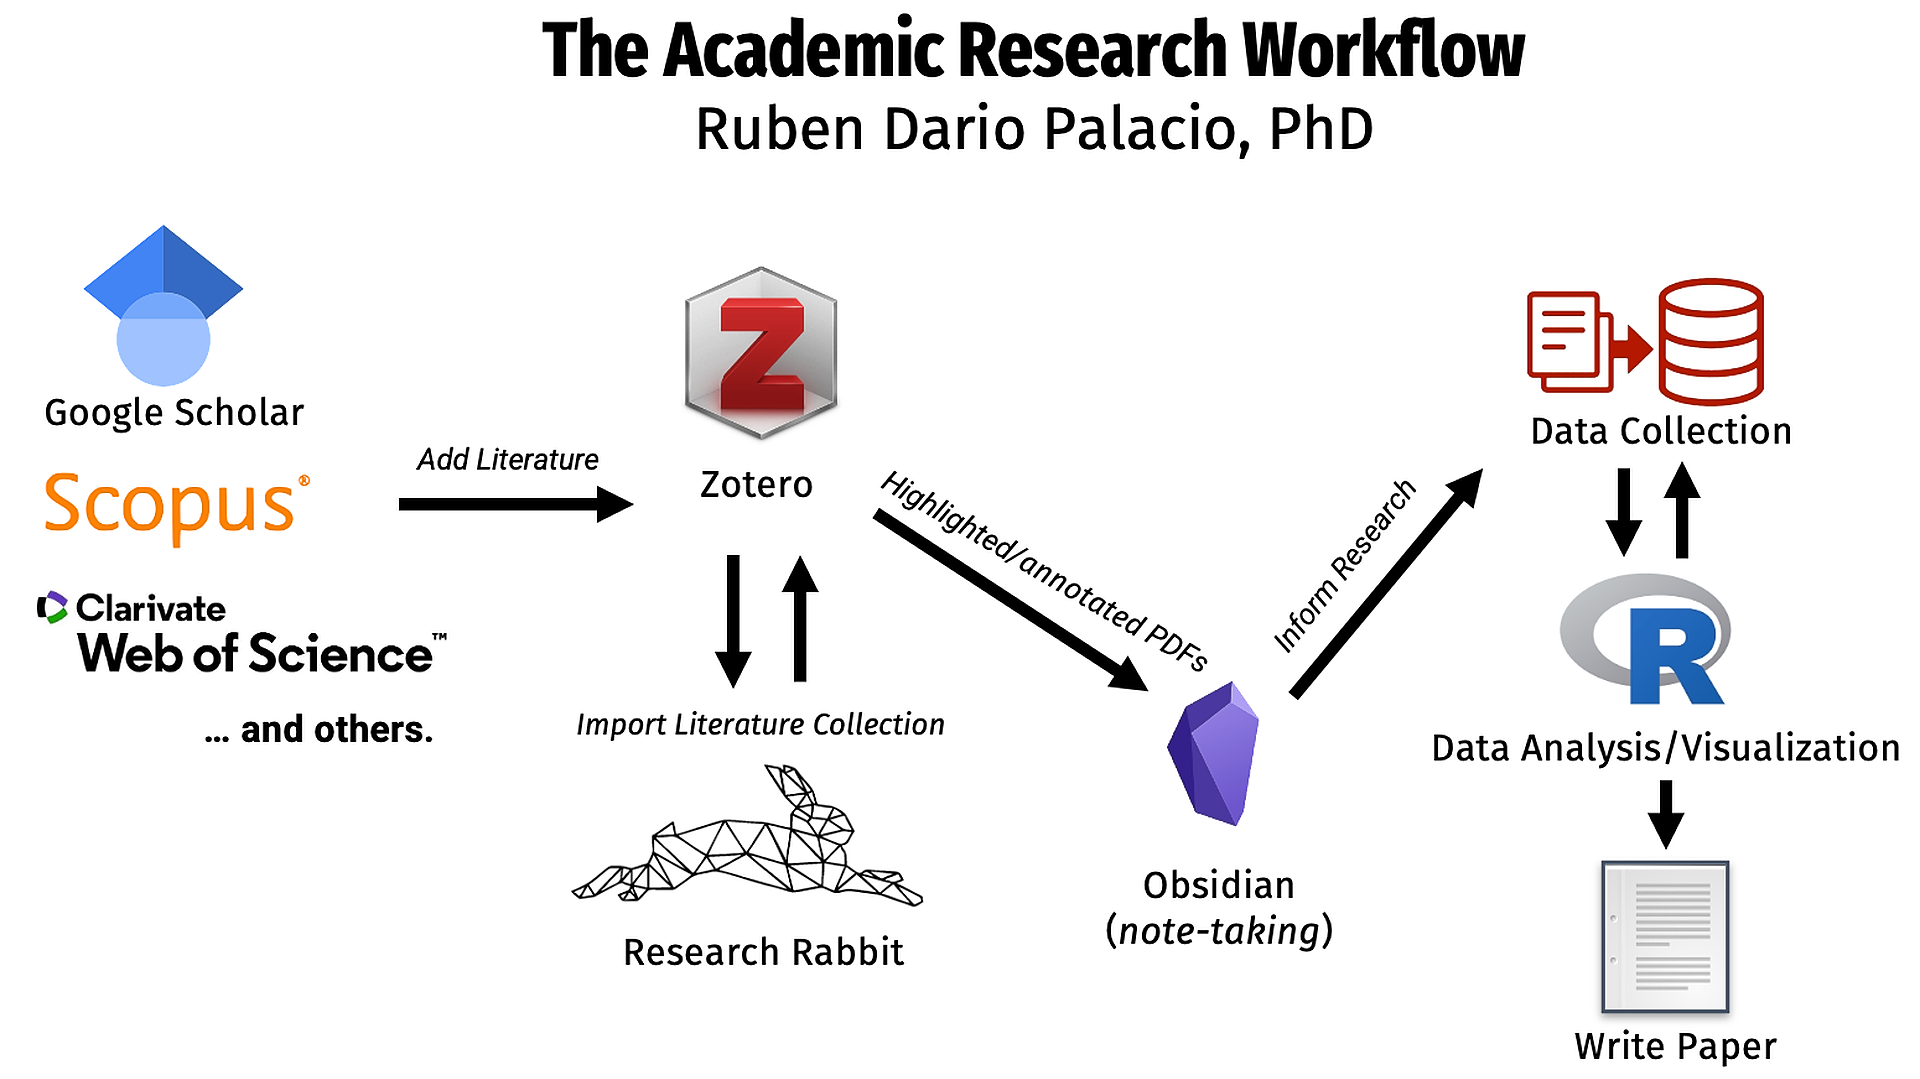
\includegraphics[width=0.9\textwidth]{./figures/analisi/diagrama.png}
\caption{Esquema simplificat del cicle entrada\,--\,procés\,--\,sortida en un treball de recerca acadèmica i en un projecte d'enginyeria.}
\label{fig:diagrama}
\end{center}
\end{figure}

El que fa singular aquest treball és precisament que opera en tots dos fluxos alhora: la implementació tècnica és l'instrument que permet respondre la pregunta de recerca, i la pregunta de recerca és la que dóna sentit a la implementació. Aquesta doble naturalesa no és una imprecisió metodològica, sinó la condició que determina com s'ha planificat i gestionat el projecte al llarg de tot el seu desenvolupament.

\section{Caràcter exploratori de la feina}
No tots els projectes neixen amb uns requisits clars i tancats. N'hi ha que, per la seva naturalesa, parteixen d'una pregunta oberta i evolucionen a mesura que els resultats intermedis revelen informació que no estava disponible a l'inici. Aquest és precisament el cas del treball que es presenta.

Un dels objectius inicials era construir un \emph{pipeline} automatitzat per generar parells d'imatges contrafactuals que poguessin servir de base per avaluar mètodes d'XAI, amb un grau de control comparable al del treball de referència \cite{Hesse2023}. L'únic criteri pactat des del principi era que el dataset fos el més fotorrealista possible; no hi havia cap decisió presa sobre quina tecnologia s'havia d'usar ni com havia de funcionar el \emph{pipeline}. Aquesta obertura defineix el caràcter exploratori del projecte.

En la pràctica, el que va succeir és que les decisions tècniques es prenien en resposta als resultats que s'anaven obtenint. El millor exemple n'és la selecció del model de generació del dataset. Inicialment, el criteri de selecció era senzill: quina tecnologia produïa imatges de millor qualitat visual. Per quantificar-ho, es van definir unes mètriques objectives que mesurien, respectivament, la similitud estructural, la magnitud del canvi i el percentatge de píxels modificats entre la imatge original i la generada. L'aplicació d'aquestes mètriques sobre els primers experiments va produir un resultat que, a priori, hauria d'haver resolt la qüestió, però no va ser així: el model que obtenia millors puntuacions en totes les tres mètriques produïa resultats perceptivament deficients si s'analitzava visualment.

Aquesta constatació va donar un nou significat a la pregunta de recerca. El treball havia deixat de ser únicament un projecte de construcció d'un dataset i validació de tècniques \ac{XAI} per convertir-se, a més, en una investigació sobre si les mètriques convencionals de qualitat d'imatge són predictors fiables de la utilitat d'un model d'\emph{inpainting} en el context de la XAI. La hipòtesi que havia guiat els primers passos, suposant que una puntuació alta en aquells indicadors implicava un millor sistema de generació d'imatges sintètiques per als propòsits del treball, havia quedat en entredit per la pròpia implementació.

La retroalimentació entre codi i hipòtesi ha estat la dinàmica natural del projecte, i reconèixer-la a temps ha estat part de la feina. Precisament perquè aquesta dinàmica era previsible des del principi, la metodologia de desenvolupament adoptada ha estat híbrida: planificant les fases i fites del procés de manera predictiva però amb certa felxibilitat a l'hora d'assolir aquestes fites per a poder absorbir els canvis de rumb sense que el projecte es desestructuri.

\section{Metodologia de desenvolupament}

L'enfocament clàssic de gestió de projectes, conegut com desenvolupament en cascada, organitza el treball en fases seqüencials i tancades: primer s'analitzen els requisits, després es dissenya, després s'implementa i finalment es valida. Cada fase assumeix que l'anterior ha quedat completament resolta abans de continuar. Aquest model funciona bé quan els requisits són estables i coneguts amb anterioritat, però és precisament el contrari del que caracteritzava aquest projecte. Aplicar \emph{Waterfall} aquí hauria significat tancar la selecció del \emph{backend} d'inpainting abans d'haver vist cap resultat real, o definir les mètriques d'avaluació XAI abans de saber quina dissociació produirien.

Per aquest motiu, la metodologia adoptada ha estat híbrida, inspirada en els principis de \emph{Scrum} però adaptada per emmarcar-la dins unes fases  estructurades. En lloc de \emph{sprints} fixos de durada predefinida, el projecte s'ha organitzat en quatre fases amb revisions periòdiques que actuaven com a punts de control naturals: al final de cada fase es revisaven els resultats obtinguts amb el tutor, es validaven les decisions preses i s'establia la direcció de la fase següent.

La primera fase ha estat la de \emph{recerca}, centrada en assolir els coneixements necessaris per abordar el treball: revisió de la bibliografia recomanada, consulta de recursos externs i formació complementària en aprenentatge profund. Aquesta fase, però, no va tenir un punt de tancament definit; la recerca ha estat una activitat transversal que s'ha mantingut activa al llarg de tot el desenvolupament, ja que cada nova fase plantejava preguntes que requerien aprofundir en la literatura.

La segona fase ha estat la d'\emph{experimentació i generació del dataset}, on es van avaluar les tecnologies candidates i, un cop seleccionada la més adequada en funció de les mètriques definides, es va construir el \emph{pipeline} automatitzat. Aquesta experimentació també es va dur a terme de forma iterativa i progressiva, amb un control sistemàtic sobre cada prova: les tecnologies avaluades es comparaven documentant les seves particularitats i generant informes que justificaven les decisions adoptades.

La tercera fase ha estat la d'\emph{avaluació XAI}, on s'han aplicat els mètodes explicatius sobre el dataset generat. Els resultats obtinguts en aquesta fase han condicionat les decisions preses sobre els models de generació, tancant el bucle de retroalimentació que caracteritza el projecte. Tot i que el flux podria semblar seqüencial, el diagrama següent il·lustra com cada fase ha retroalimentat les anteriors.

\begin{figure}[h]
\begin{center}
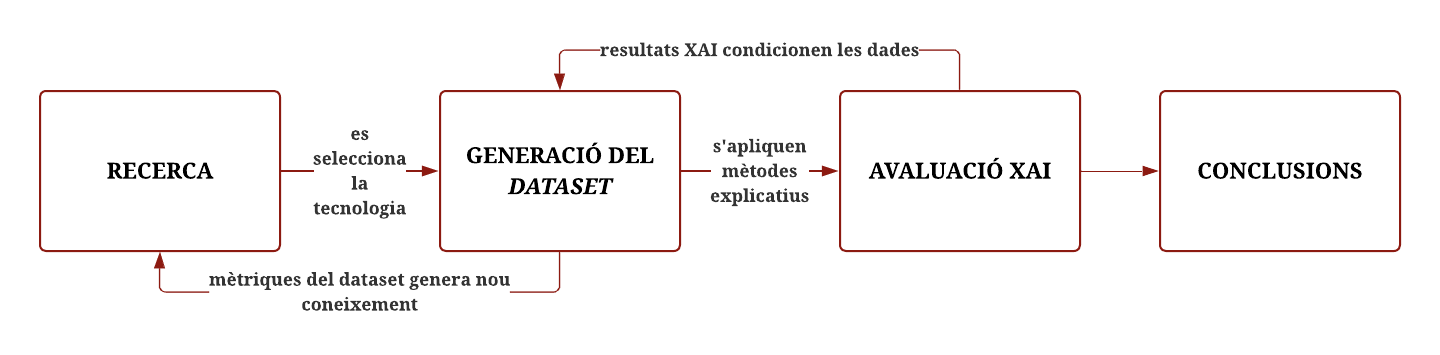
\includegraphics[width=0.9\textwidth]{./figures/analisi/workflow.png}
\caption{Flux continu de retroalimentació del projecte.}
\label{fig:workflow}
\end{center}
\end{figure}

Finalment, la quarta fase ha estat la de \emph{redacció}, on els resultats i decisions de les fases anteriors s'han documentat i contextualitzat en forma de memòria. Aquesta fase, igual que la de recerca, s'ha solapat parcialment amb les anteriors: la redacció dels capítols tècnics ha anat avançant en paral·lel amb l'experimentació, de manera que els raonaments quedaven documentats alhora.

\section{Planificació, riscos i eines}
Definida la metodologia de desenvolupament, cal concretar com s'ha materialitzat en la pràctica: quines fases s'han planificat, quins riscos s'han identificat i amb quines eines s'ha dut a terme la gestió del projecte.

\subsection{Planificació temporal}

El treball s'ha estructurat en quatre fases principals, cadascuna amb un conjunt de tasques associades i un lliurable que en marcava el tancament. La planificació no ha estat rígida: les fases han tingut una durada flexible i, en alguns casos, s'han solapat parcialment entre elles. La fase de recerca, per exemple, ha estat activa durant tot el desenvolupament, i la redacció ha avançat en paral·lel amb l'experimentació durant les darreres etapes.

Les quatre fases s'han succeït de manera aproximadament seqüencial, però amb retroalimentació entre elles. La fase d'exploració de tecnologies va precedir necessàriament la construcció del \emph{pipeline}, ja que la selecció del \emph{backend} condicionava tota la implementació posterior. L'experimentació XAI, al seu torn, no podia començar fins que el dataset fos suficientment gran i consistent. I la redacció, tot i concentrar-se a les etapes finals, ha acompanyat el procés des del principi: documentar s'han generat varis informes dels experiments realitzats per evitar la pèrdua d'informació rellevant sobre el raonament que els va motivar.

\subsection{Fites i lliurables}
Cada fase del projecte ha tingut associat un lliurable concret que en certificava la finalització i servia de base per a la revisió amb el tutor. Aquesta pràctica ha obligat a materialitzar els resultats intermedis en alguna cosa tangible i revisable en forma d'informe, evitant que les fases s'allarguin indefinidament sense un criteri de tancament clar.

Les fites principals del projecte han estat les següents. La primera, al final de la fase de recerca, va ser un \emph{informe comparatiu de tecnologies} que documentava els experiments inicials amb unes tecnologies de generació primerenques i les mètriques comparatives dels resultats. La segona fita va ser el \emph{pipeline funcional}: un sistema automatitzat i reproduïble capaç de generar parells contrafactuals a partir d'un dataset establert, calcular les mètriques per parell i exportar els resultats. La tercera fita va ser el conjunt de resultats obtinguts després d'aplicar un classificador sobre les dades generades i l'aplicació d'un model explicatiu. Finalment, la quarta fita és la \emph{memòria}, que documenta i contextualitza tot l'anterior.

\subsection{Gestió de riscos}
Tot projecte comporta incerteses que cal identificar i gestionar. En el cas d'aquest treball, tres riscos principals han condicionat les decisions preses al llarg del desenvolupament.

\begin{enumerate}
\item \emph{Dependència d'APIs externes}: l'ús de models de software propietari per a establir-ne la comparació implica una dependència d'un servei de tercers amb un cost econòmic variable per generació. Per mitigar aquest risc, es va tenir en compte com a prioritari l'ús de models oberts, reproduïbles pel públic i que fossin disponibles per a la comunitat de recerca. 

\item \emph{Cost computacional}: el refinament del classificador i la generació en local del dataset sobre el volum d'imatges parelles objectiu podrien requerir un temps de procés considerable. 

\item \emph{Qualitat i mida del dataset}: un dataset massa petit o amb parells de baixa qualitat podria invalidar les conclusions de l'experiment XAI. Per mitigar-ho, es van definir criteris de filtratge estrictes sobre les imatges i es va establir com a objectiu una mida de $\sim$500 parells, una xifra informada pel treball de referència \cite{Hesse2023}.
\end{enumerate}

\subsection{Eines de gestió}
La gestió del projecte s'ha recolzat en tres eines principals, cadascuna cobrint una necessitat diferent. \emph{Notion} ha estat el centre de planificació i la base de coneixement. S'hi han gestionat els experiments del projecte, s'ha documentat la bibliografia consultada i s'han registrat algunes de les decisions tècniques preses durant el desenvolupament. La flexibilitat de l'eina, que permet combinar taules relacionals i pàgines de notes dins d'un mateix espai de treball, l'ha fet especialment adequada per a un projecte amb una estructura que ha evolucionat al llarg del temps.

\begin{figure}[h]
\begin{center}
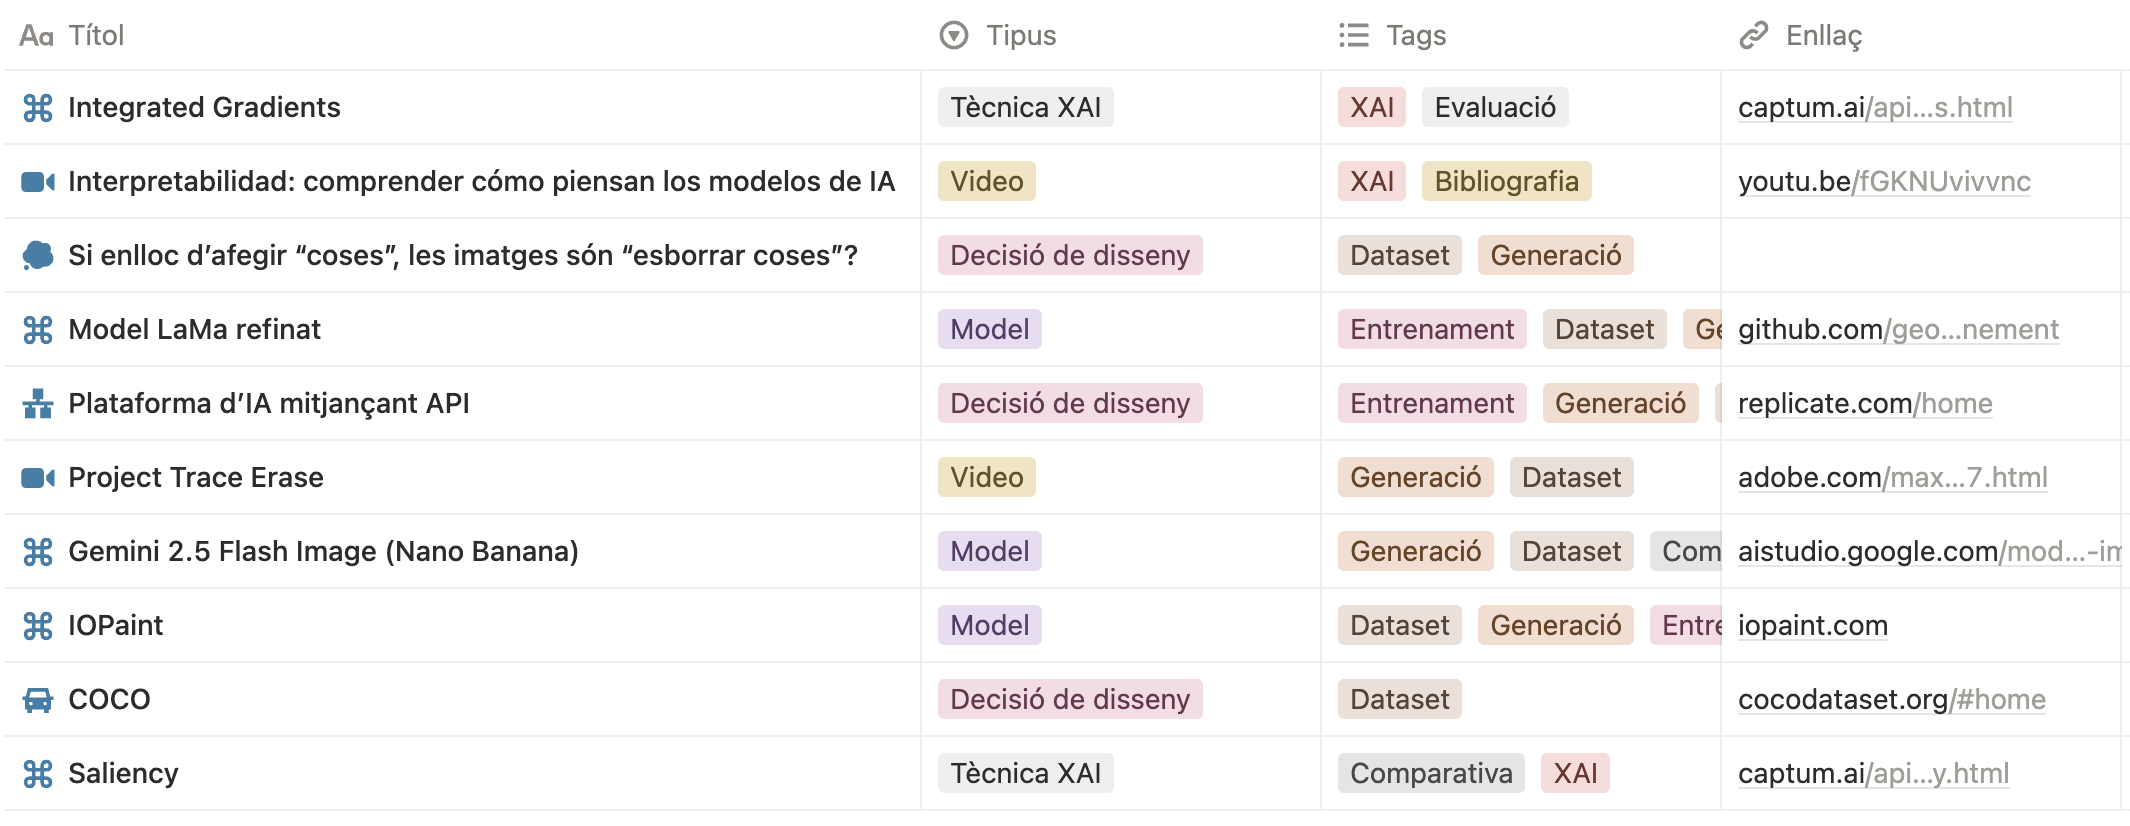
\includegraphics[width=0.9\textwidth]{./figures/analisi/knowledge.png}
\caption{Captura de pantalla de la BBDD de Notion}
\label{fig:knowledge}
\end{center}
\end{figure}

\emph{GitHub} ha exercit de sistema de control de versions per a tot el codi del projecte. A més de la funció habitual de registre de canvis, ha permès mantenir un historial clar de les decisions d'implementació i ha facilitat la recuperació de versions anteriors en els moments en què un canvi de rumb ho requeria. 

Finalment, \emph{Overleaf} ha estat l'entorn de redacció de la memòria i els informes intermigs, permetent treballar en \LaTeX de tal manera que gran part de la documentació corresponent a la fase d'experimentació s'ha redactat orientada al format final de la memòria.